\section{Numerical Integration}

To numerically calculate a integral of a function $f$. We can
use the trapezoidal rule \cite{trapezoidal}. The trapezoidal rule 
approximates the area under a graph of a function as a trapezoid and 
calculates the area. This can be done for more and more trapezoids to increase
accuracy but also coming at a computational cost. The trapezoidal rule can 
approximate a definite integral with riemann sums by splitting the interval 
$[a, b]$ such as $a < x_0 < x_1 < \dots < x_{N-1} < x_N$ and perform the 
following calculation

\begin{equation}
    \int_a^b f(x) \, dx \approx \frac{\Delta x}{2} \left(f(x_0) + 2f(x_1) + \cdots + 2f(x_{N-1}) + f(x_N)\right)
\end{equation}

The sum in this calculation does not depend on each other and can therefore be
parallelized and calculated independently and summed up when they are complete.
This has been implemented in our code by creating a C++ program that takes in
the command line arguments $N$ for the no of threads and $T$ for the no of
trapezoids. All threads gets $\frac{N}{T}$ trapezoids besides the last unlucky
thread that gets $\frac{N}{T} + T \Mod N$ due to ease of implementation. All
the threads operate this function and work on a shared variable to calculate 
the sum, hence the mutexes.

\begin{lstlisting}[language=C++, caption=non-determinism.cpp]
void *calculateFactorial(void *conf)
{
  Config *cfg = (Config *)conf;
  double localResults;

  for (int i = 0; i < cfg->numTrapPerThread; i++)
  {
    int pos = cfg->startI * cfg->numTrapPerThread + i;
    if (pos == 0 || pos == numTrapezes)
    {
      continue;
    }
    localResults = localResults + 2 * function(a + ((pos)*w));
  }

  results_mutex.lock();
  results += localResults;
  results_mutex.unlock();

  pthread_exit(0);
}
\end{lstlisting}

\subsection{Experimental Results}

\begin{figure}
  \centering
  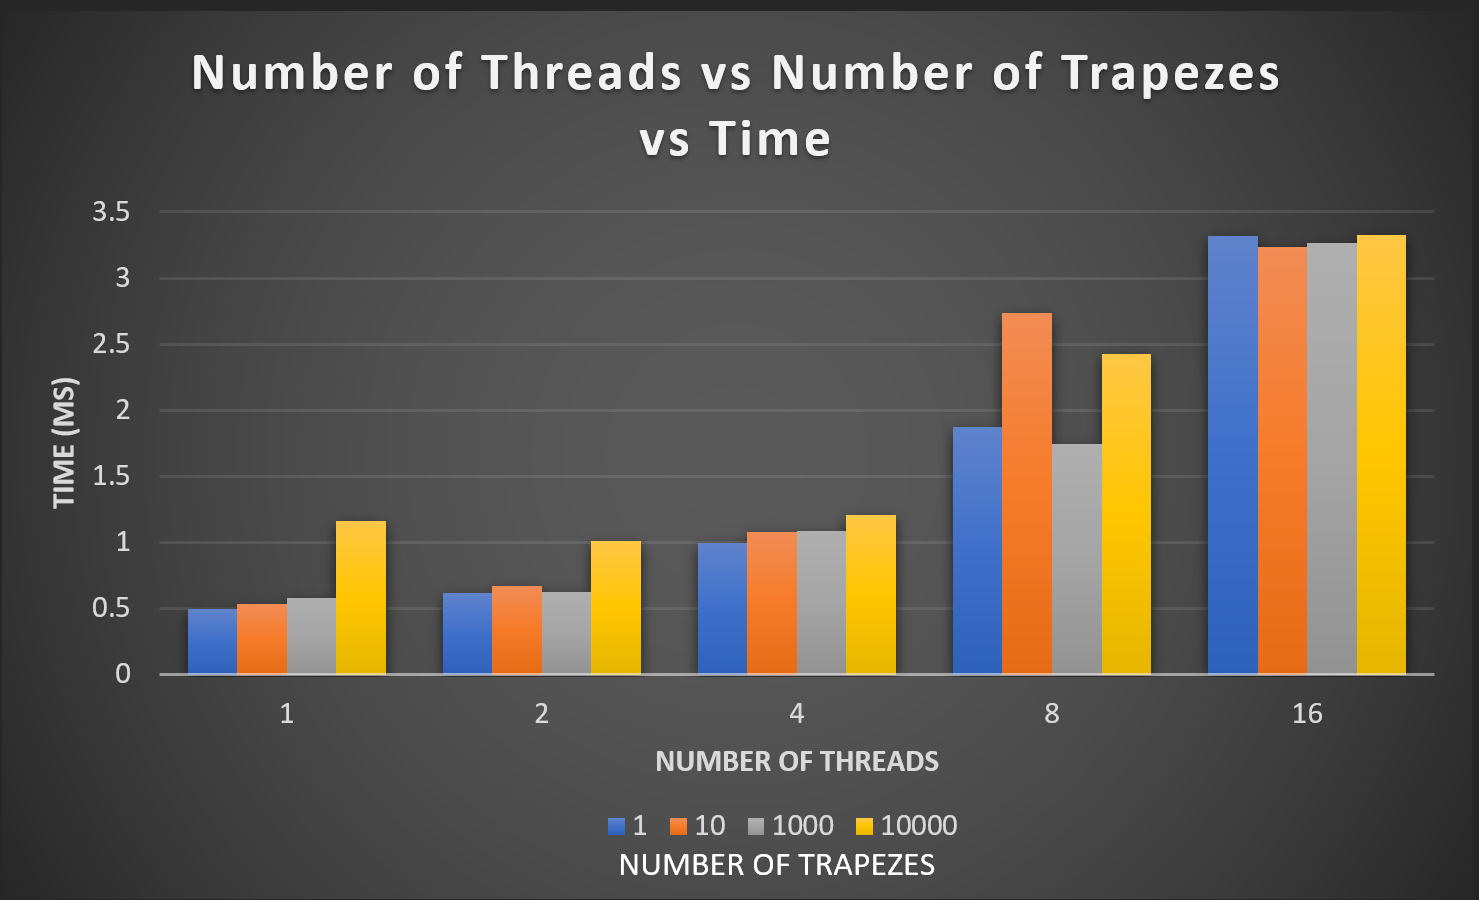
\includegraphics[width=\linewidth]{Figures/lowTrap.png}
  \caption{Different simulations for $T<10000$ and $N \in \{1, 2, 4, 8, 16\}$}
  \label{fig:lowtrap}
\end{figure}

As threads increased for low amount of trapezes, the time to compute actually 
increases shown in figure \ref{fig:lowtrap}. This is due to the overhead that 
parallelization adds to the application (thread-creation, waiting on threads 
to complete and lock-waits). However as we reach medium amount of trapezes 
($10^6$ in figure \ref{fig:medtrap}) or high ($10^9$ in figure \ref{fig:hightrap}) we see that the time decreases significantly as 
at this point the cost to parallelize is less than the benefit it offers. 
While the number of trapezes increase, so too did the accuracy of the result.

\begin{figure}
  \centering
  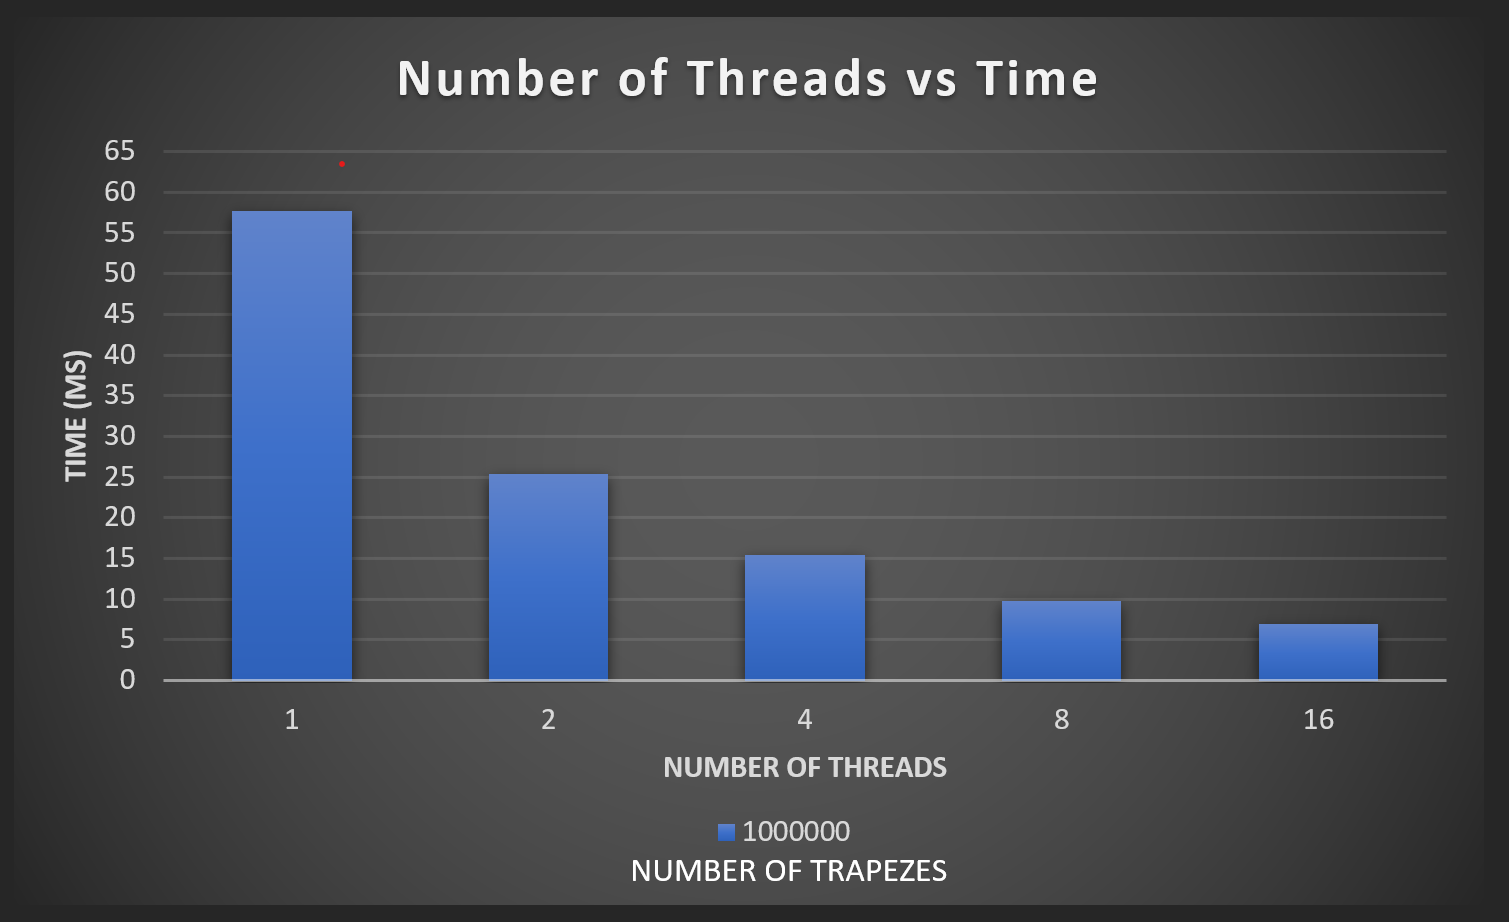
\includegraphics[width=\linewidth]{Figures/medTrap.png}
  \caption{Different simulations for $T=10^6$ and $N \in \{1, 2, 4, 8, 16\}$}
  \label{fig:medtrap}
\end{figure}

\begin{figure}
  \centering
  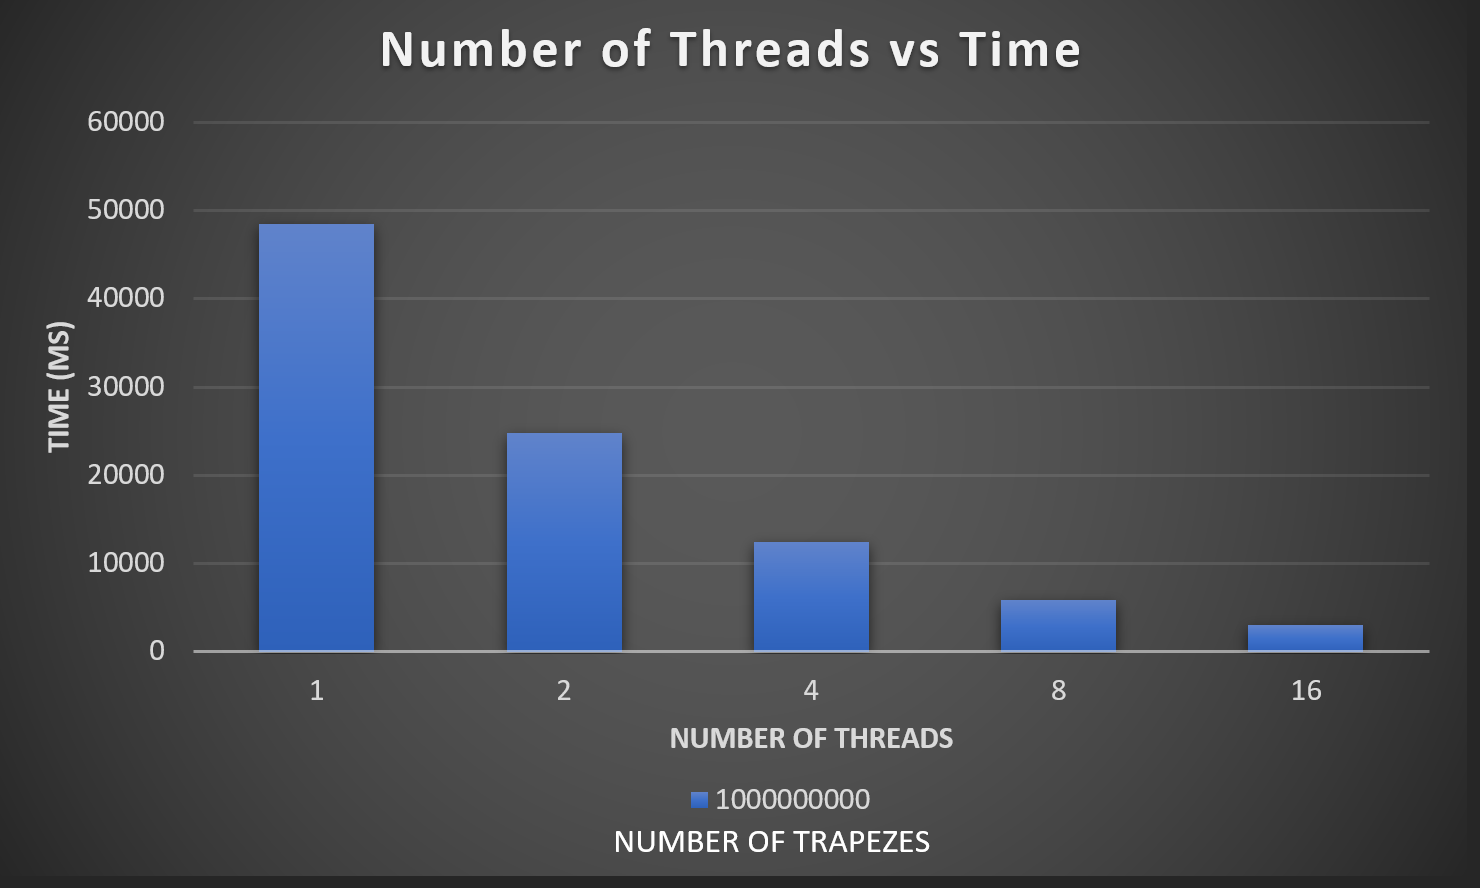
\includegraphics[width=\linewidth]{Figures/highTrap.png}
  \caption{Different simulations for $T=10^9$ and $N \in \{1, 2, 4, 8, 16\}$}
  \label{fig:hightrap}
\end{figure}

\subsection{Evaluation}
This solution takes a very naive approach to parallelizing the program. 
It attempts to split the number of trapezes by the number of threads
(with the surplus going to the last thread). This means that:

\begin{itemize}
  \item the work load is not evenly split (in terms of the data partitioning)
  \item the time taken for each thread to complete varies based on the effort 
  required to complete the calculation for a given trapeze.
\end{itemize}

An improvement to speed can occur if a thread queueing system was implemented 
instead, where each thread worked on a single trapeze (until max threads).
Thereafter as a thread completed, a new thread would spin up and compute the 
next trapeze. This would ensure that no thread would be wasted, as until the 
sum was complete, all threads would be working (in a more equal and more 
efficient manner). However the queuing solution could potentially have a mutex 
related bottle neck as result would need to be written after computing a single 
trapeze area (vs in our solution, it is only written at the end of a set of 
trapezes).
